\documentclass[12pt,a4paper]{jsreport}
\usepackage{bm}
\usepackage[dvipdfmx]{graphicx}
\usepackage{ascmac}
\usepackage[hang,small,bf]{caption}
\usepackage[subrefformat=parens]{subcaption}
\captionsetup{compatibility=false}
\usepackage{geometry}
% ページの余白を1.25インチにする
\geometry{
    left=1.25truein,
    right=1.25truein,
    top=1.25truein,
    bottom=1.25truein,
}
\usepackage{etoolbox}
\patchcmd{\chapter}{\cleardoublepage}{}{}{}
\patchcmd{\chapter}{\clearpage}{}{}{}

\title{埋設されたパイプの位置・方向推定のための\\偏波感受型圧縮センシング}
\author{\\指導教員    廣瀬明教授 \\              夏秋嶺准教授\\
03-210499   高原陽太
}


\begin{document}
\maketitle
\tableofcontents
\clearpage
\chapter{はじめに}
\section{研究背景}
 工事のための地中調査を行う際、地中の埋設物の有無及びその状態を特定することは必須である。
特にガス管や水道管などが道路工事現場に埋まっているものの代表例として
挙げられる。そこで実際に工事を施工する前の調査段階でそれら埋設物の詳しい情報を得ておくことが重要となる。
\\ そのため電波を利用して地中を非破壊的に探知する地中レーダ(GPR)探査技術が用いられる。GPRは地中埋設物探査や遺跡調査、地下水流
調査など多くの応用分野を持つ\cite{radar1}\cite{radar2}。特定周波数帯の電磁波を地中に照射しその散乱特性を見る。
\\ 仕組みは以下の通りである。電磁波は地中を伝搬し、土壌中にて誘電率が異なる物質の境界面で散乱を起こす。そのため埋設物の材料物質と
土壌の誘電率の違いを利用して埋設物の検知を行う。


\begin{figure}[h]
    \begin{center}
     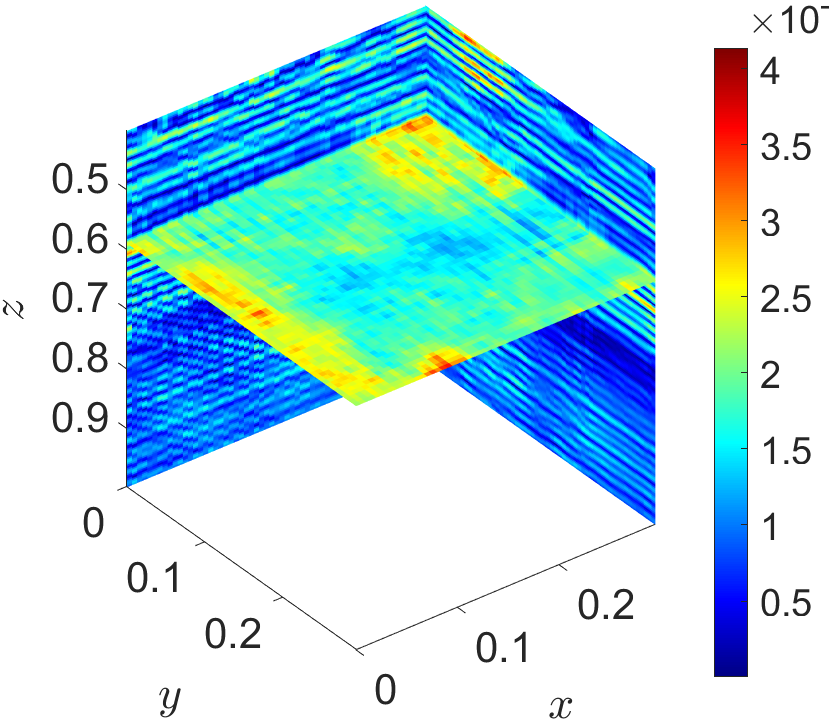
\includegraphics[width=7cm]{./image/0918.png}
     
    \caption{鉄パイプをGPRによって可視化したもの}\label{鉄パイプをGPRによって可視化したもの}
    \end{center}
    \end{figure}

 また、GPRの基本的な装置として一対の送受信アンテナを地面に照射するものがある。しかしこの場合地表全体で
多数の計測を行うため膨大な時間が必要である。ゆえに計測の時間を減らす方法が検討されてきた。そのため少ない計測点
から本来の信号を復元する圧縮センシングと呼ばれる手法が用いられる。この手法によってより少ない時間で埋設物を推定すること
ができる。加えてこの埋設物を推定する上でその物体がパイプ状でありかつ延伸の向きが分かれば、さらに探索が高速化すると考えられる。

\section{研究の目的}
 本研究の目的はガス管や水道管などの線状物体をモデル化し、偏波依存性を用いることで地中に埋設されているパイプ管の有無と向きをより少ない計測点
で推定することである。そのため偏波依存型の圧縮センシングを提案し、実験によりその有用性を検証する。

\chapter{関連技術}
\section{地中レーダの原理}
 地中レーダは電磁波の地下物体からの
散乱を利用した地下計測手法である。地表に置かれた送信アンテナ
から電磁波パルスを地中に放射し、受信アンテナで受信する。地中を伝搬する電磁波は、土壌中に
誘電率が異なる物質が存在すると散乱を起こす性質を持ち、そのため埋設物の誘電率
と土壌の誘電率の違いを利用して埋設物の存在を検知することが可能となっている。この散乱の様子から
埋設物が埋まっている位置と深度を計測する。
\\ 地中では電磁波速度は導電率、誘電率、透磁率によって決まる。しかし透磁率はほぼ一定であり、GPRでは10MHzより高い
周波数領域で計測が行われるため、地下媒質の電気的性質は比誘電率$\varepsilon$にのみ左右される。
この時の地中伝搬速度$v$は

\begin{equation}
  v =
  \frac{c}{\sqrt{\varepsilon}} 
  \end{equation}

と書ける。

そして地中の伝搬速度が分かりさえすれば、送信電波が散乱して戻ってくる時間
$\tau$を計測することで図\ref{地中レーダの様子}のように物体の深度$d$は次式で導出できる。
    \begin{equation}
        d=
        \frac{v \tau}{2} 
    \end{equation}

また同様に反射波の振幅も誘電率によって推定できる。図\ref{地中レーダの様子}のように
誘電率の異なる二層媒質構造の場合について考える。この時上層から入射する電波は境界面で反射を受け
、振幅比$\Gamma$の反射波が発生する。

    \begin{figure}[h]
        \begin{center}
            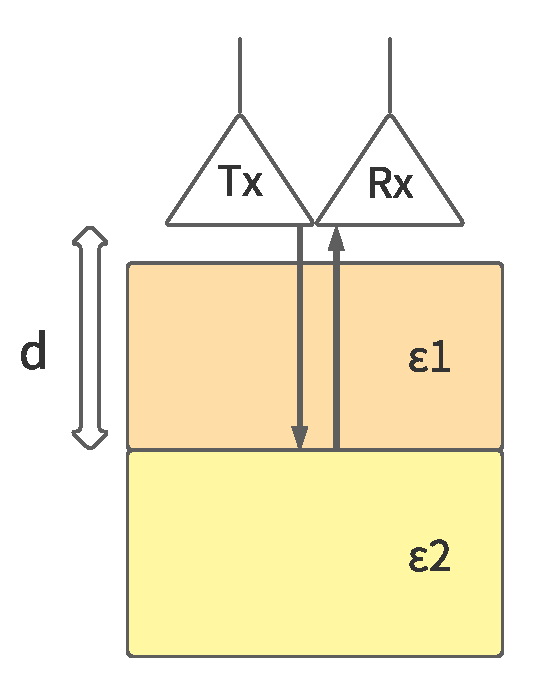
\includegraphics[width=7cm]{./image/antenna_depth_2.pdf}

            \caption{地中レーダの様子}\label{地中レーダの様子}
        \end{center}
    \end{figure}

反射係数$\Gamma$は境界面で以下のように与えられる。
\begin{equation}
  \Gamma=
  \frac{\sqrt{\varepsilon_{1}}-\sqrt{\varepsilon_{2}}}{\sqrt{\varepsilon_{1}}+\sqrt{\varepsilon_{2}}} 
\label{gamma}  
\end{equation}


式(\ref{gamma})は反射係数が二つの媒質の誘電率のみによって決まることを示している。これらの情報を測定することで埋設物の位置と材質を推定する。
\\
\\ また実際の地中レーダの受信波形には送信アンテナから直接受信アンテナに届く直達波、地表面で反射される地表反射波
が混在してしまう。そのため地中反射波を強調するには直達波と地表反射波を取り除く必要がある。


\section{電磁波と偏波}
 偏波とは図\ref{偏波のイメージ}のように電界と磁界が直行しながら伝搬する波における電界の向きのことを指す。電磁波を用い、目標物に
照射することで散乱波から目標物に関する情報を得ることができるため、GPRにも用いられている。単に埋設物の散乱係数の振幅だけで
なく位相の情報も利用することができるという利点を持つ。
todo:ここをフルポラリメトリ用に書きなおす。
\\ 特に埋設物がパイプなどの線状物体である時に偏波の状態を観測することは重要になる。というのも図\ref{偏波方向とパイプの向きによる反射強度の違い}
のように電磁波の偏波方向と線状物体の方向が一致するときに大きな散乱が起こるのに対して、偏波方向が線状物体と直行すると散乱が非常に小さくなってしま
うからである。ゆえにパイプを検出する際には偏波の向きと計測対象の向きを一致させることが必要となる。
\begin{figure}[h]
  \begin{center}
   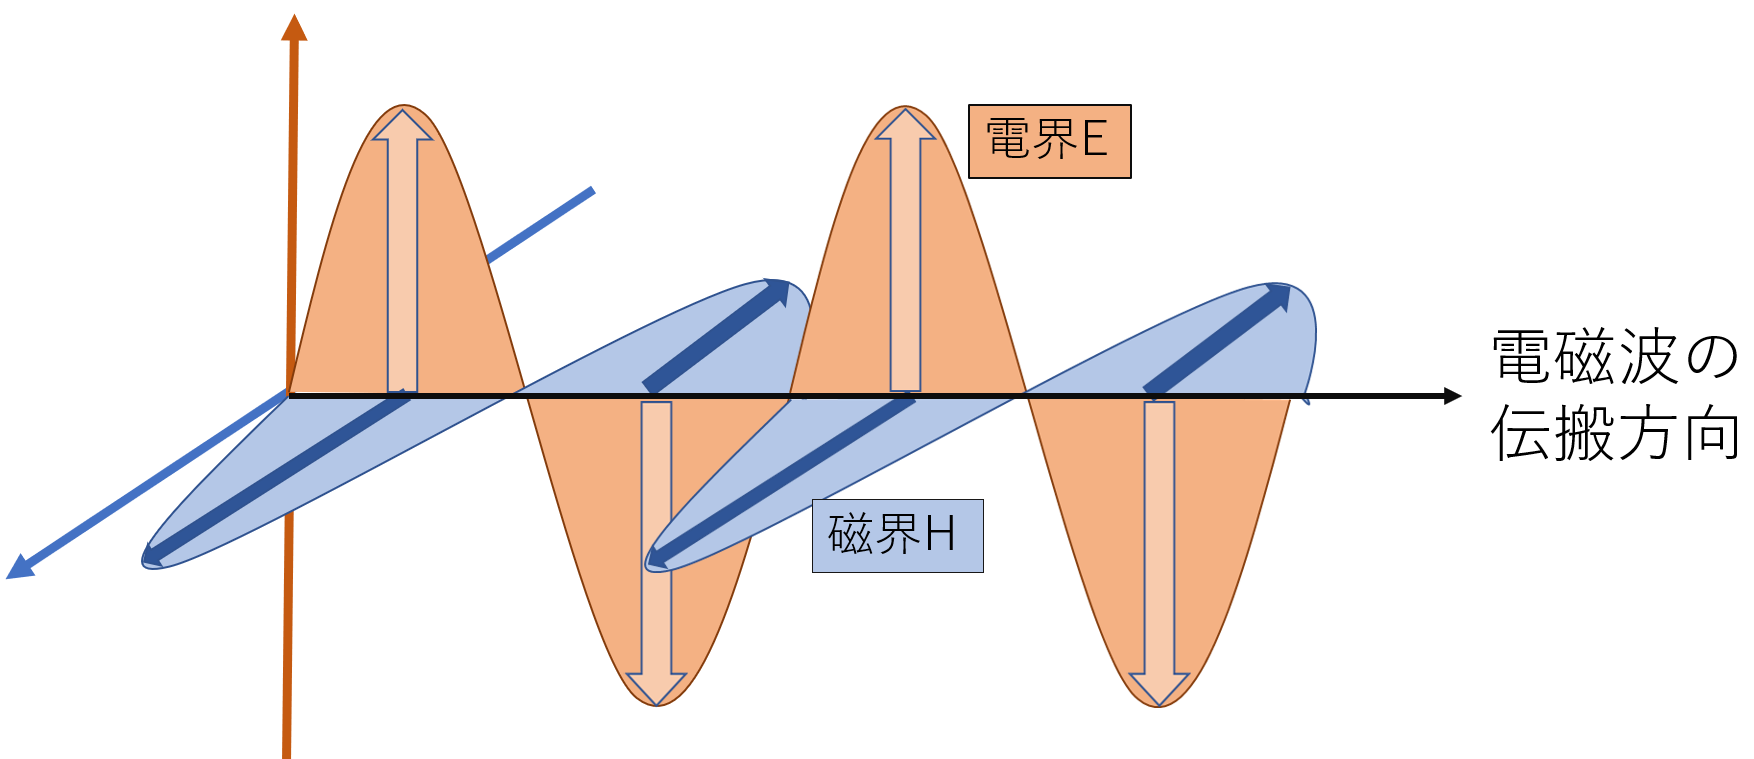
\includegraphics[width=10cm]{./image/wave_propagation.png}
  \caption{偏波のイメージ}\label{偏波のイメージ}
  \end{center}
  \end{figure}

  \begin{figure}[h]
    \begin{center}
     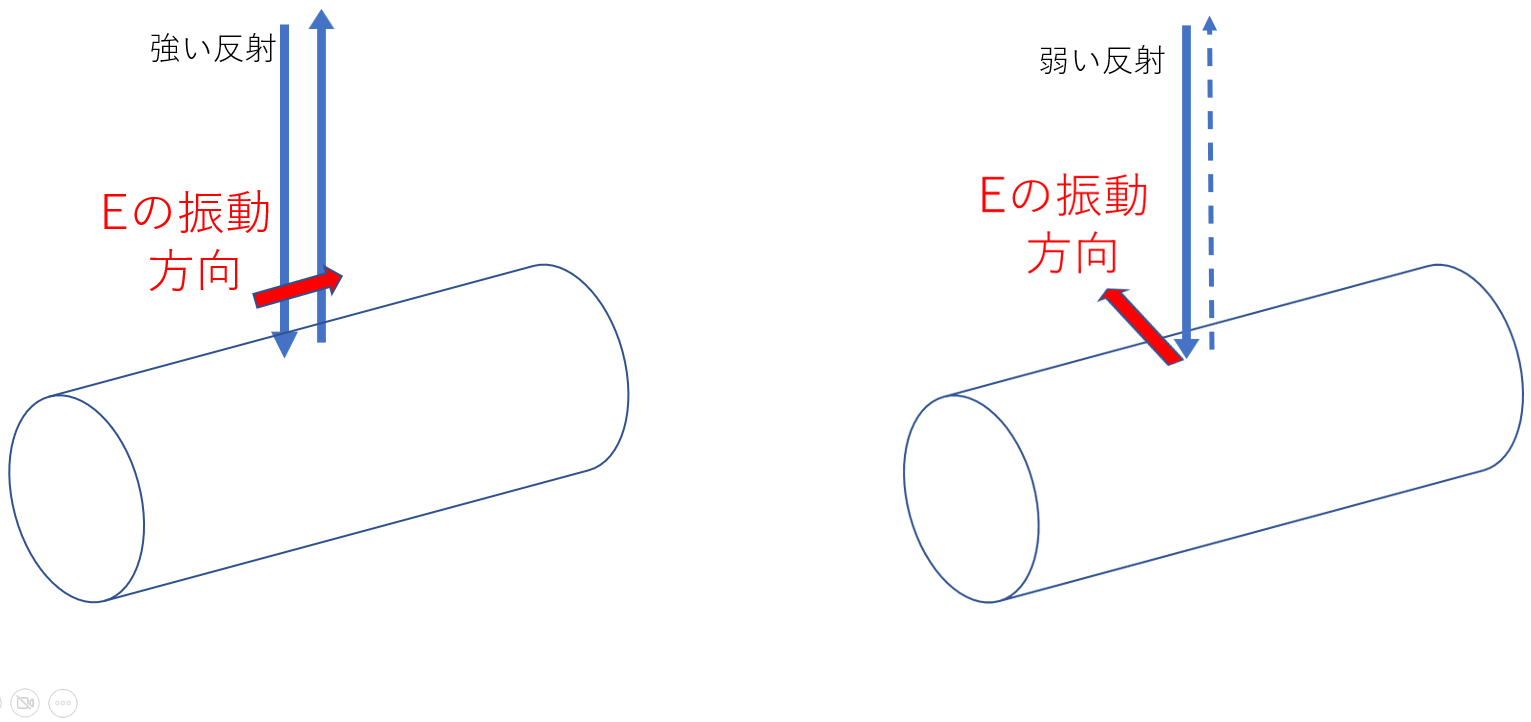
\includegraphics[width=10cm]{./image/final.png}
    \caption{偏波方向とパイプの向きによる散乱強度の違い}\label{偏波方向とパイプの向きによる反射強度の違い}
    \end{center}
    \end{figure}


\section{圧縮センシングとモデル内一様性による圧縮}
 圧縮センシングとは、対象となる信号をできるだけ少ない観測点数から本来あるべき密なデータを抽出する技術のことである。まばらな計測点から
密なデータを構成することで、データ観測にかかる時間を短縮することを可能とする。
\\ また一様性に着目することでセンシングの対象から得られる散乱のパワーだけでなく、位相などの様々な情報を用いることが可能となり、
圧縮センシングを拡張することができる\cite{imai}。そこではその内部が一様性を持つような
モデルを仮定する。目標物の領域内でその性質が均一ならばその散乱特性も変わらない、すなわち一様であると考えられる。
このモデルを計測領域で空間的に掃引し、目標物を検知する。
モデルの位置と目標物の位置が一致したとき、その領域内では散乱特性は一様になり、領域外では散乱特性は一様とならない。
このことを利用して地中の目標物をその形や大きさを含めて検出することができる。


\chapter{提案手法}
\section{従来の手法}
 地中埋設物、主に地雷の検知のためにGPRが用いられている。しかし計測点が多数になり計測時間が膨大になってしまう。todo:ここらへんの記述適当
\\ また、これらの手法のほとんどが散乱の強度を用いたものであった。しかし強度のみの情報では目的の埋設物とその他関係がない埋設物との区別が困難になってしまう。
\\ 強度以外の情報を用いた手法として\cite{hirose1}~\cite{hirose3}にあるようにテクスチャなどの高次元な計測情報を特徴量として用いたものが挙げられる。
この手法では各計量点において空間、周波数領域における相関を含む特徴量ベクトルを構成する。それらのベクトルは自己組織化マップによって分類される。
\\ また\cite{imai}では地中に埋まっている地雷を模した円柱型のプラスチック模型を探知する際に円形のモデルを仮定して圧縮センシングを行っている。
\\ この手法について紹介したい。まず計測点数を考えるときにスパース性を利用すると少ない点数で済む。これは測定して得られた信号にゼロ成分が多いという条件付け
をすることで計測データを減らせるという圧縮センシングの考えに基づく。
\\ todo:ここ合ってるん?次に空間座標$(x_{i},y_{i})$から位置ベクトル$\bm{r}=(x_{i},y_{i})$を定め、$h(\bm{r_{m}})$を円形モデルによる予想値と位置$\bm{r_{m}}$での計測値との一致度合とする。この時、
\begin{equation}
  \bm{h} =
      \left[
      \begin{array}{rrrr}
      h(\bm{r_{m1}})&h(\bm{r_{m2}})&h(\bm{r_{m3}})&\cdots
      \end{array}
      \right]^\mathrm{T}
      \label{mbh}
  \end{equation}
% \begin{equation}
%   $\bm{h}$ =
%         \left[
%         \begin{array}{rrr}
%         h(\bm{r_{m1}})&h(\bm{r_{m2}})&\cdots
%       \end{array}
%         \right]
%     \end{equation}


このベクトル$\bm{h}$を一様性ベクトルと考える。
\\ まばらな計測結果による散乱係数を$\bm{s_{0}}$とする。これを$\bm{h}$ができるだけスパース性を満たすように繰り返し更新し、実際の密計測データ$\bm{s}$を推定する。そこで
$p$($0<p<1$)を用いて評価関数$f(\bm{h})$を次式のように定める。
\begin{equation}
  f(\bm{h})=\sum_{l}|h(\bm{r_{ml}})|^{p}
  \end{equation}

関数$f(\bm{h({\bm{s}})})$の$\bm{s}$に関する勾配を求め、ステップ幅$\alpha_{t}$を用いて$\bm{s_{t}}$を更新する。
\begin{equation}
  \bm{s_{t+1}}=\bm{s_{t}}-\alpha_{t}\nabla_{\bm{s}}*f(\bm{s_{t}})
  \end{equation}

として評価関数$f$が十分収束するまで$\bm{s}$の更新を行い、最終的に$h(\bm{r_{m}})$が極大を示す場所$\bm{r_{m}}$に目標物が埋まっていると考えられる。この手順に
よってまばらな点数での計測を可能にしている。



\section{提案手法todo:ここ大分書き換える}
 従来手法のようにパイプ管をモデル化し、それによって圧縮センシングを行うことを提案する。パイプ管をモデル化する際にまず文献\cite{imai}のように一様とみなせる領域を考える。パイプのような線状の物体は線方向に一様である。
ゆえに線状方向に関しては計測点数を減らすことが可能となる。
\\ それゆえパイプの向きを推定することが必要となる。しかし実際にGPRを用いた時、図\ref{電波の散乱の様子}のようにパイプにぶつかった電磁波はあらゆる方向に散乱し、また
図\ref{偏波方向とパイプの向きによる反射強度の違い}のように電界の向きによって散乱波の振幅が大きく異なる。
\\ そのため例えばパイプの向きに垂直に偏波を照射してしまった場合、散乱の大きさによって埋設物を検知するGPR上ではパイプの存在を検知しにくい。
よって向きがわかってないパイプをGPRによって計測する場合、偏波の向きを水平、垂直どちらに対しても行う必要がある。

\begin{figure}[h]
  \begin{center}
   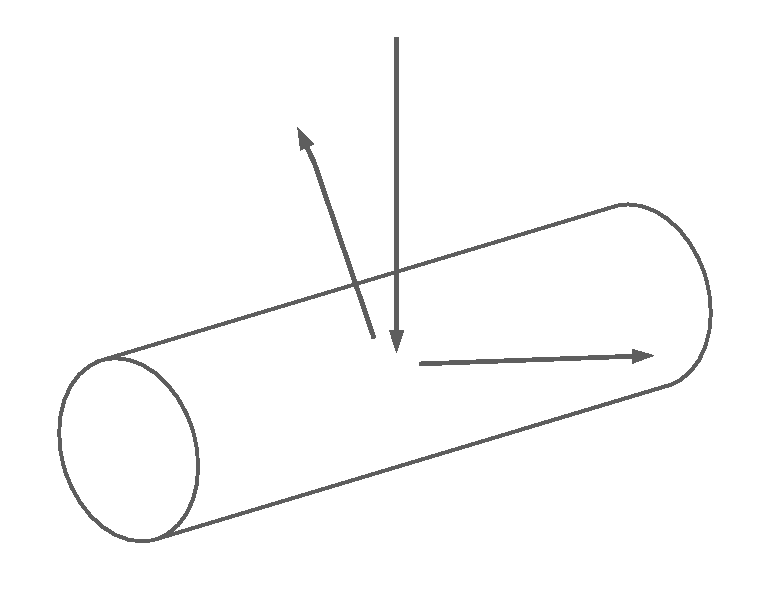
\includegraphics[width=7cm]{./image/scattering.pdf}
  \caption{電波の散乱の様子}\label{電波の散乱の様子}
  \end{center}
  \end{figure}

 逆に言えば、偏波を水平、垂直に照射し、散乱波の強さを比較することでパイプの向きがより水平方向あるいは垂直方向
か分かる。ゆえにデータ処理の際、ある測定点での散乱波の偏波依存性からパイプの向きが推定でき、
その方向への測定点数を減らすことに繋がる。よって圧縮センシングを行う際、偏波の情報を加味することでより
測定時間の短縮が期待できると考える。
\\ この時フルポラリメトリを用いてデータ取得を行う。すなわち水平偏波(H)、垂直偏波(V)の二通りを送信し、水平、垂直のアンテナ
で受け取ることにより4通りのデータを取得するようにする。これを式で表すと、散乱行列は式(\ref{フルポラリメトリ})のようになる。

\begin{equation}
  S =
      \left[
      \begin{array}{rrr}
      S_{HH} & S_{HV}  \\
      S_{VH} & S_{VV} 
      
      \end{array}
      \right]\label{フルポラリメトリ}
  \end{equation}
この散乱行列を従来手法の散乱係数と置き換え、式(\ref{mbh})をパイプの向きも考慮したものにすることで上記手法を実現する。
理論の詳細はこれから整備する。









\clearpage

\begin{thebibliography}{99}
    \bibitem{radar1}M.Sato and M.Takeshita,”Estimation of subsurface fracture roughness by
    polarimetric borehole radar,” IEICE Trans. Electron., E83-C,12(2000) 1881-1888
    \bibitem{radar2}T.Moriyama, M.Nakamura, Y.Yamaguchi and H.Yamada,”Radar polarimety applied
    to the classification of target buried in the underground: Wideband Interferometric
    Sensing and Imaging Polarimetry,” Vol.3210 of Proc. of SPIE(1997) 182-189
     \bibitem{phasor}K.Oyama and A.Hirose, "Phasor Quaternion Neural Networks for Singular
     Point Compensation in Polarimetric-Interferometric
     Synthetic Aperture Radar," IEEE Transactions on Geoscience and Remote Sensing, vol. 57, no. 5, May 2019.
     \bibitem{human detection}Y.Kim, and T.Moon, "Human Detection and Activity Classification Based
     on Micro-Doppler Signatures Using Deep
     Convolutional Neural Networks," IEEE Geoscience and Remote Sensing Letters, vol. 13, no. 1, January 2016.
     \bibitem{imai}R.Imai, Y.Song, R.Natsuaki, and A.Hirose, IEEE Transactions on Geoscience and Remote Sensing,
     "Model-Based Homogeneity to Extend Compressed Sensing for Ground Penetrating Radar," vol. 60, 2022.
     \bibitem{hirose1}Y.Nakano and A.Hirose, “Improvement of plastic landmine visualization performance by use of ring-csom and frequency-domain local
     correlation,” IEICE Transactions on Electronics, vol.E92-C, no.1,
     pp.102-108, 2009.
     \bibitem{hirose2}Y.Nakano and A.Hirose, “Adaptive identification of landmine class
     by evaluating the total degree of conformity of ring-SOM,” Australian
     Journal of Intelligent Information Processing Systems, pp.22-28,2010. %http://ajiips.com.au/papers/V12.1/AJIIPS_vol12n1_26-31.pdf
    \bibitem{hirose3}R.Natsuaki and A.Hirose, “Circular property of complex-valued
    correlation learning in CMRF-based filtering for synthetic aperture
    radar interferometry,” Neurocomputing, vol.134, pp.165-172, 2014.
   %  https://www.sciencedirect.com/science/article/pii/S092523121400126X
   
    
     
     % \bibitem{jireishuu}https://geology.co.jp/archives/projects/%E5%9C%B0%E4%B8%AD%E3%83%AC%E3%83%BC%E3%83%80%E3%83%BC%E3%81%AE%E6%96%B0%E3%81%9F%E3%81%AA%E4%BA%8B%E4%BE%8B%E9%9B%86%EF%BC%88%E3%82%B1%E3%83%BC%E3%82%B9%E3%82%B9%E3%82%BF%E3%83%87%E3%82%A3%EF%BC%89#case01
   
     % \bibitem{satou}http://cobalt.cneas.tohoku.ac.jp/users/sato/newpage24.htm#:~:text=%E5%9C%B0%E4%B8%AD%E3%83%AC%E3%83%BC%E3%83%80%E3%81%AF%E9%9B%BB%E7%A3%81%E6%B3%A2,%E3%83%91%E3%83%BC%E3%82%BD%E3%83%8A%E3%83%AB%E3%83%BB%E3%82%B3%E3%83%B3%E3%83%94%E3%83%A5%E3%83%BC%E3%82%BF%E3%81%A7%E8%A8%98%E9%8C%B2%E3%81%99%E3%82%8B%E3%80%82
     % \bibitem{cs}https://www.innervision.co.jp/ressources/pdf/innervision2014/iv201409_061.pdf
    
     \end{thebibliography}

\end{document}